\section{Verification}

\begin{figure}[ht] 
    \centering
    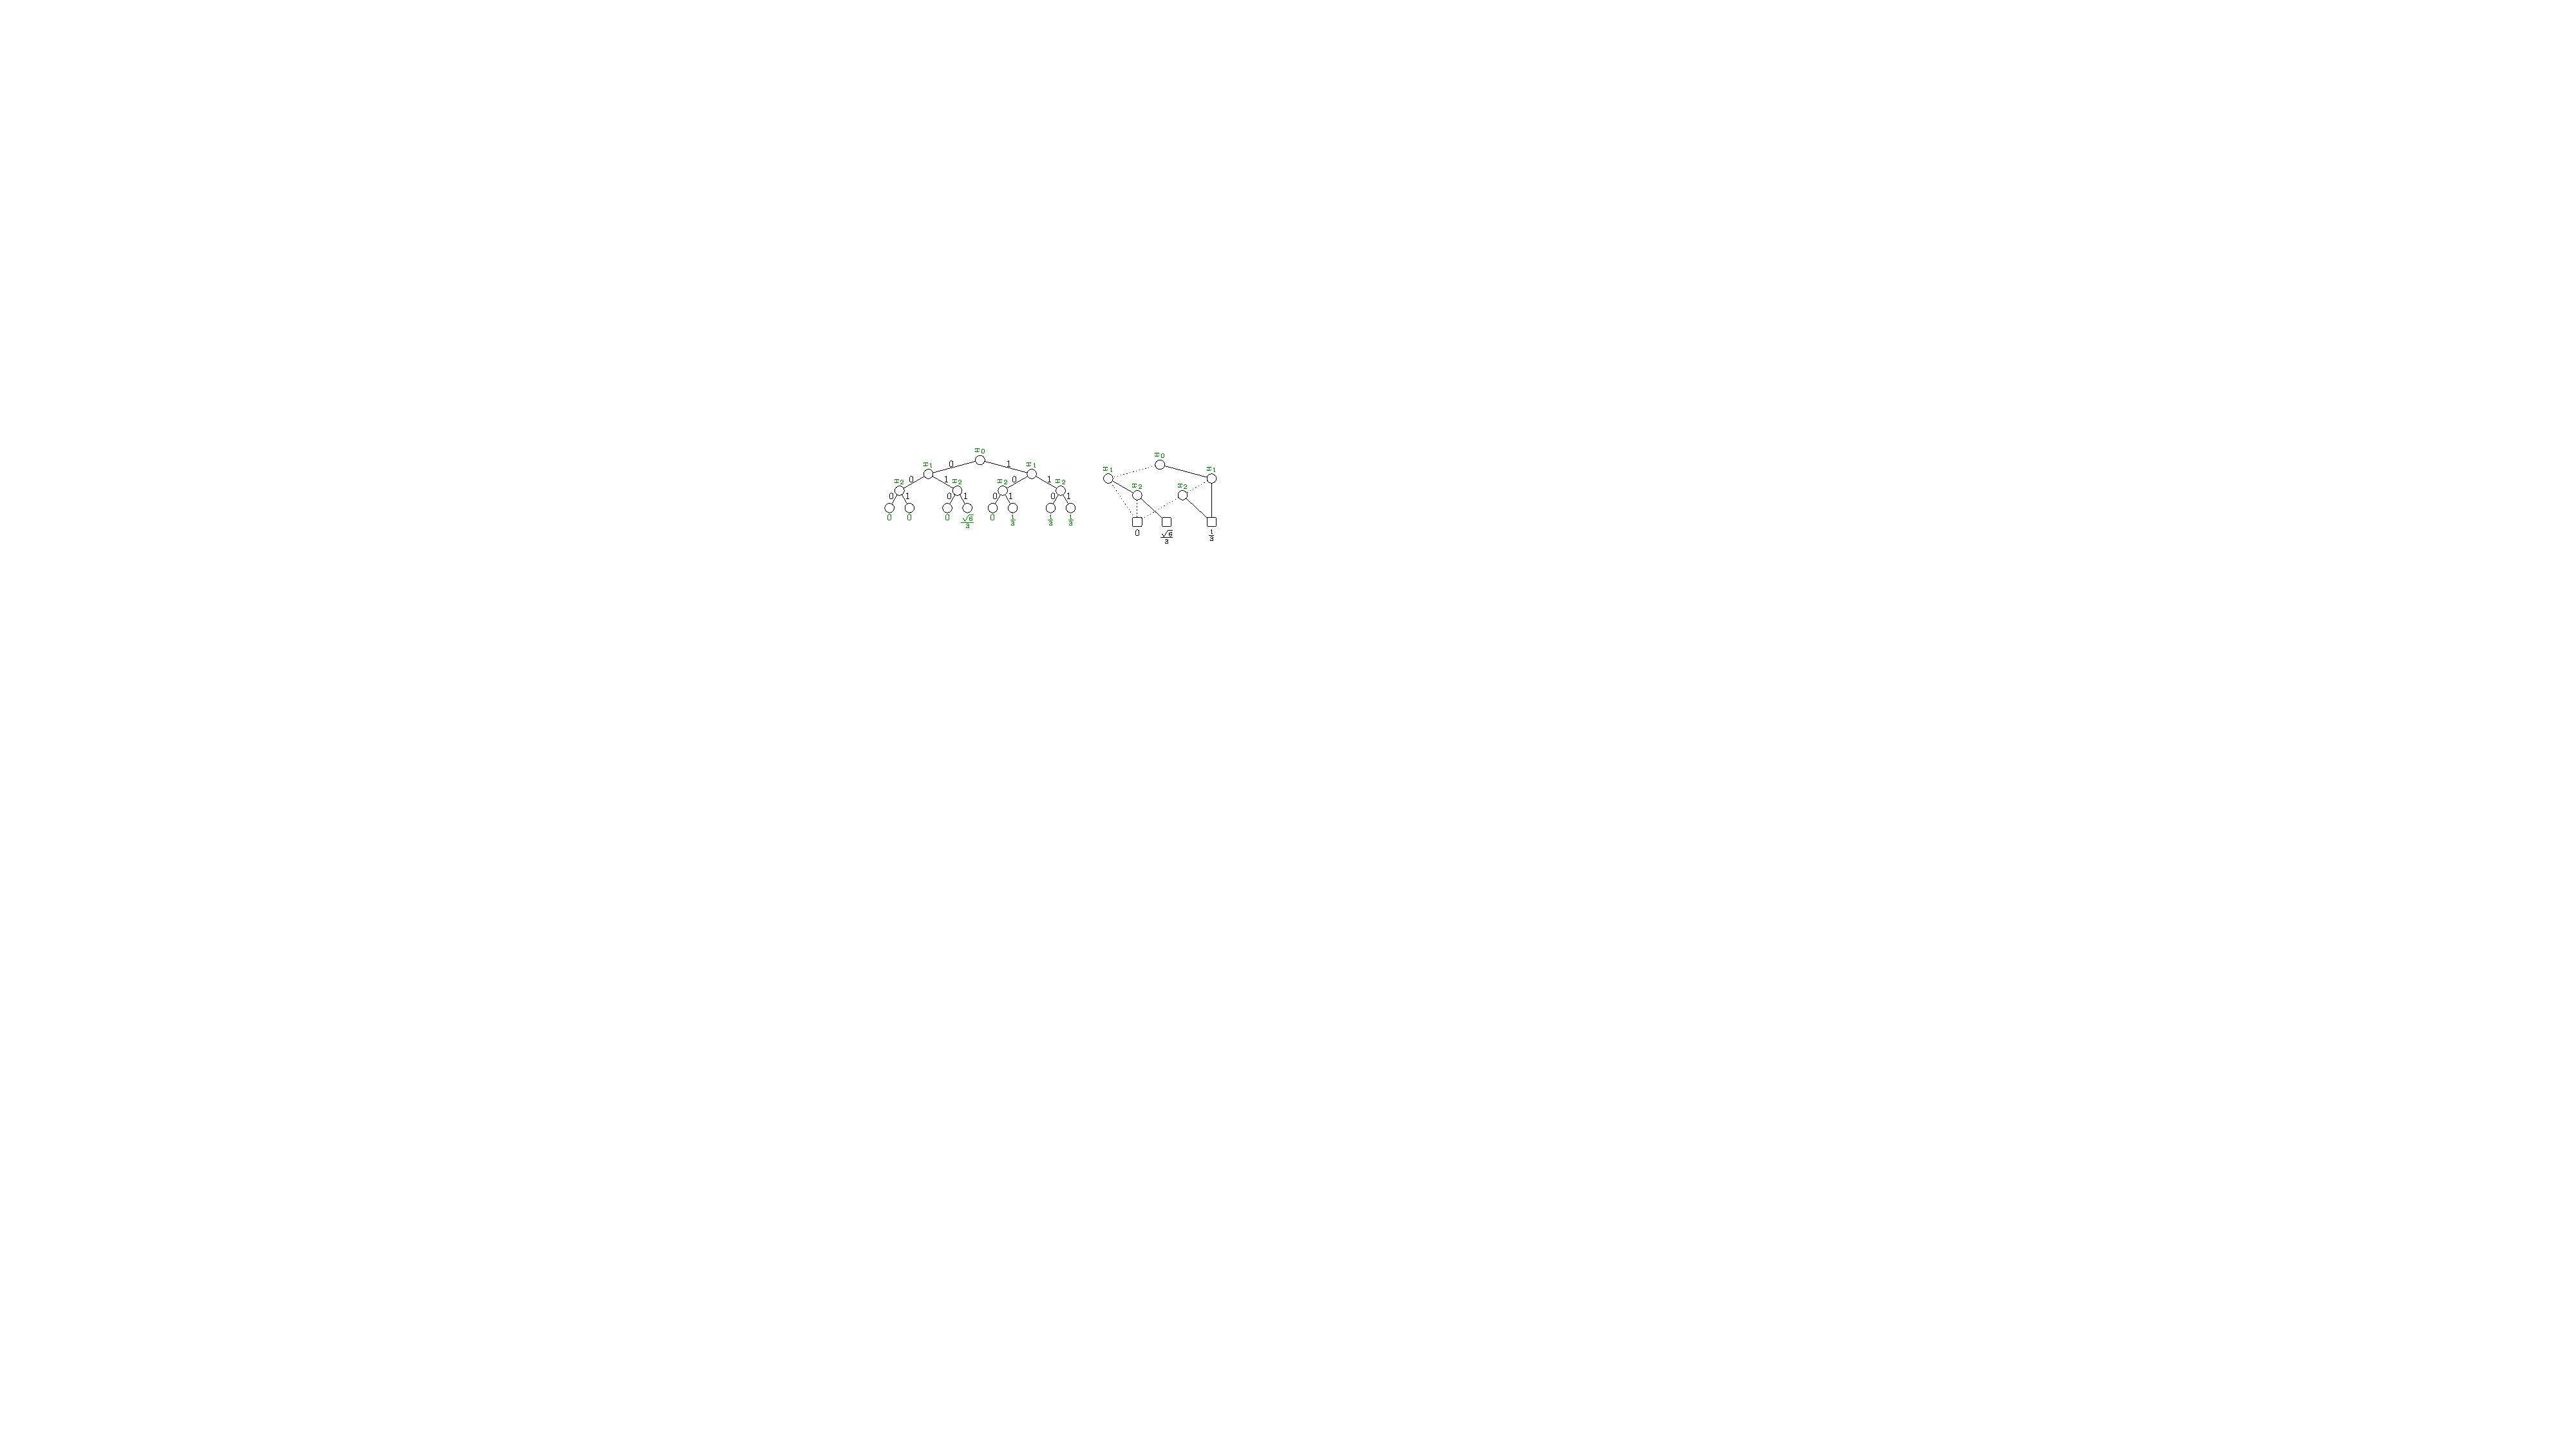
\includegraphics[scale=0.9]{Figures/BDDs/BDDs} 
    \caption{The BDD representation of a quantum state..}
    \label{BDD:fig}
\end{figure}
%
We can formulate the {\it program verification} problem as an instance of the classical Hoare's Logic
\[
P \{C\} Q
\]
where $P$ is the {\it pre-condition}, $Q$ is the post-condition, and $C$ is a program.
%
The pre-condition $P$ characterizes a set of {\it initial} ({\it source}) states, and the post-condition $Q$ characterizes a set of {\it final} ({\it target}) states.
%
We would like to verify that if we execute $C$ from any state satisfying $P$, then we end up in state satisfying $Q$.
%
Here, take $C$ to be a quantum circuit.
%
A fundamental breakthrough in the verification of conventional computer systems, was the invention of efficient data structuires to represent  
